%% Supplementary material for the JRSS-A submission (OUP authoring template)
%% (modern, medium, single column, numbered headings, author-year references).
%% The working draft with the same content is main.tex.
\documentclass[namedate,webpdf,modern,medium]{oup-authoring-template}
\onecolumn

\usepackage{mathtools}
\usepackage{bm}
\usepackage{bbm}
\usetikzlibrary{arrows.meta}

\newcommand{\indep}{\protect{\perp\!\!\!\perp}}
\newcommand{\given}{\mid}
\newcommand{\RR}{\mathbb{R}}
\DeclareMathOperator*{\argmax}{arg\,max}

% Alternative text for figures, as required by the journal (shown under each
% caption in the submitted manuscript, not in the typeset article).
% Switch: \showalttexttrue for the submission, \showalttextfalse to hide them.
\newif\ifshowalttext
\showalttexttrue
\newcommand{\alttext}[1]{\ifshowalttext\par\smallskip{\footnotesize\noindent Alt text: #1}\fi}

\graphicspath{{./}}
\newcommand{\societylogo}{}

\begin{document}

\journaltitle{Journal of the Royal Statistical Society Series A: Statistics in Society}
\DOI{DOI added during production}
\copyrightyear{2027}
\pubyear{2027}
\access{Published: Date added during production}
\appnotes{Supplementary Material}
\firstpage{1}

\title[Defensive coverage schemes from tracking data]{Supplementary Material for ``Integrating Unsupervised and Supervised Learning for the Prediction and Interpretation of Defensive Schemes in American Football''}

\author[1]{Rouven Michels}
\author[2]{Robert Bajons}
\author[3]{Jan-Ole Fischer}

\address[1]{\orgdiv{Department of Statistics}, \orgname{TU Dortmund University}, \orgaddress{\postcode{44221} \state{Dortmund}, \country{Germany}}}
\address[2]{\orgdiv{Institute for Statistics and Mathematics}, \orgname{WU Vienna University of Economics and Business}, \orgaddress{\state{Vienna}, \country{Austria}}}
\address[3]{\orgdiv{Department of Business Administration and Economics}, \orgname{Bielefeld University}, \orgaddress{\state{Bielefeld}, \country{Germany}}}

\abstract{This supplement contains the selection of the initial distribution and of the lag of the hidden Markov model, the list of model features, and the predicted random effects of the defensive teams.}

\keywords{American football, forecasting, hidden Markov model, random effects, XGBoost}

\maketitle

%\stitle{Supplementary Material}
%\sdescription{Supplementary Material to}
\section{Initialization of the state distribution}

To obtain an informed initialization of the assignments between offensive and defensive players at the beginning of each play, we adopt a probabilistic matching approach based on the vertical distances between players. Specifically, for each defender \( i \) and each of the \( N = 5 \) potential offensive players \( j \), we compute a similarity score using a softmax over the negative distances,
\[
\delta_{ij} = \frac{\exp(-\alpha \, |\mathrm{y}^{(\text{def})}_i - \mathrm{y}^{(\text{att})}_j|)}{\sum_{k=1}^{n_{\text{att}}} \exp(-\alpha \, |\mathrm{y}^{(\text{def})}_i - \mathrm{y}^{(\text{att})}_k|)} \, ,
\]
where \( \mathrm{y}^{(\text{def})}_i \) and \( \mathrm{y}^{(\text{att})}_j \) denote the vertical positions of defender \( i \) and offensive player \( j \), respectively.  
The parameter \( \alpha > 0 \) controls the sharpness of the resulting distribution: higher values of \( \alpha \) yield nearly deterministic one-to-one assignments, while smaller values produce smoother, more uncertain matchings. This choice reflects the intuition that defenders tend to align with the nearest offensive player at the start of the play. We chose $\alpha$ by profile likelihood with the homogeneous version of the HMM on a random subset of 1,000 plays at lag $l = 4$. Table~\ref{tab:alpha} shows that the likelihood is maximal at $\alpha = 4$, which we use in the full model. The play-level HMM features hardly depend on $\alpha$: their correlations with the features for $\alpha = 1$ are at least 0.988 for $\alpha = 4$ and at least 0.96 for $\alpha = 16$.

\begin{table}[ht]
\centering
\caption{Profile likelihood of the sharpness $\alpha$ of the initial distribution (homogeneous HMM, lag 4, 1,000 plays): difference in the negative log likelihood to the best value, and correlation of the play-level HMM features with those for $\alpha = 1$.}
\label{tab:alpha}
\begin{tabular}{rrccc}
\hline
$\alpha$ & $\Delta$ nll & \multicolumn{3}{c}{Correlation with features for $\alpha = 1$} \\
 & & Exp.\ switches & Exp.\ \# switching defenders & Mean entropy \\
\hline
0.25 & 2279.0 & 0.999 & 0.998 & 0.998 \\
0.5 & 1064.3 & 0.999 & 0.999 & 0.999 \\
1 & 351.4 & 1 & 1 & 1 \\
2 & 47.7 & 0.998 & 0.998 & 0.999 \\
4 & 0 & 0.990 & 0.988 & 0.993 \\
8 & 50.0 & 0.978 & 0.971 & 0.984 \\
16 & 109.9 & 0.971 & 0.961 & 0.976 \\
\hline
\end{tabular}
\end{table}  

\section{Lags}
\begin{table}[ht]
\centering
\caption{AIC of the homogeneous HMM for different lags $l$ (see Eq.~(3) of the main manuscript) relative to the best model (1,000 plays, 265,990 observations).}
\label{fig:lags}
\begin{tabular}{lrrrrrrr}
\hline
Lag $l$ & 0 & 1 & 2 & 3 & 4 & 5 & 6 \\
\hline
$\Delta$AIC & 4618 & 2931 & 1579 & 614 & 93 & 0 & 348 \\
\hline
\end{tabular}
\end{table}

To determine an appropriate lag value $l$, we conducted a preliminary analysis using a homogeneous HMM. This decision was made separately from the full model design to avoid unnecessarily increasing the computational complexity. Lags ranging from $l=0, \ldots, 6$ were fitted on the same observations of a random subset of 1,000 plays, and the corresponding models were evaluated based on the Akaike Information Criterion (AIC) (see Table~\ref{fig:lags}). Lags of four and five frames are clearly preferred over shorter and longer lags (similar to \citealp{wu2023evaluation} in soccer). Their difference is small, and in a second subset of 500 plays, the order of the two was reversed ($\Delta$AIC of 30 in favour of $l=4$). The difference of 93 in AIC corresponds to a log-likelihood difference of about 46, which is very small relative to the 265,990 observations, and reaction times of 0.4 and 0.5 seconds are substantively equivalent. We therefore use $l=4$ in all subsequent analyses.

\section{Feature engineering and model features}
\label{app:features}

Prior to more involved feature engineering steps, we transform the coordinate system by redefining the x-variable as the x-distance to the end zone (such that all play directions are from right to left and the relevant end zone is at zero), and changing the direction, such that zero degrees represents heading straight towards the corresponding end zone. As mentioned in the main document, we use player features from five defensive and five offensive players. First, we standardized their $x$- and $y$-coordinates with respect to the football and ordered the players according to their $y$-coordinates, i.e., the first defender in our dataset is always the leftmost defensive player, while the first offensive player is always the rightmost one (offensive play direction is from left to right). A detailed list and description of all features used for modelling defensive coverage can be found in Table \ref{tab:variables}. %Note that initially, we extracted an even larger number of features containing information on the orientation and direction of the players, however due to small number data points, and resulting problems such as overfitting, we refrained from incorporating these features in the final analysis. 


\begin{table}[ht]
\centering
\tiny
\caption{Model features and descriptions.}
\label{tab:variables}
\resizebox{\linewidth}{!}{
\begin{tabular}{p{5cm} p{10cm}}
\hline
\textbf{Feature group} & \textbf{Description} \\
\hline

$\text{Convex hull area}^{\dagger}$ &
Area of the convex hull formed by player positions.
Includes:
\texttt{chull\_area\_o} (offense),
\texttt{chull\_area\_d} (defense). \\

$\text{Convex hull span (x-coordinate)}^{\dagger}$ &
Spread of the convex hull in x-coordinate direction.
Includes:
\texttt{chull\_x\_o} (offense),
\texttt{chull\_x\_d} (defense). \\

$\text{Convex hull span (y-coordinate)}^{\dagger}$ &
Spread of the convex hull in y-coordinate direction.
Includes:
\texttt{chull\_y\_o} (offense),
\texttt{chull\_y\_d} (defense). \\

$\text{Relative x-position of offensive players}^{\dagger}$ &
Relative x-coordinates of individual offensive players with respect to the football.
Includes:
\texttt{x\_rel\_player\_off1} to \texttt{x\_rel\_player\_off5}. \\

$\text{Relative x-position of defensive players}^{\dagger}$ &
Relative x-coordinates of individual defensive players with respect to the football.
Includes:
\texttt{x\_rel\_player\_def1} to \texttt{x\_rel\_player\_def5}. \\

$\text{Relative y-position of offensive players}^{\dagger}$ &
Relative y-coordinates of individual offensive players with respect to the football.
Includes:
\texttt{y\_rel\_player\_off1} to \texttt{y\_rel\_player\_off5}. \\

$\text{Relative y-position of defensive players}^{\dagger}$ &
Relative y-coordinates of individual defensive players with respect to the football.
Includes:
\texttt{y\_rel\_player\_def1} to \texttt{y\_rel\_player\_def5}. \\

$\text{Down}^{\dagger}$ &
Current down of the play (1st, 2nd, 3rd, or 4th down). \\

$\text{Quarter}^{\dagger}$ &
Game quarter in which the play occurs. \\

$\text{Yards to go}^{\dagger}$ &
Distance in yards required to achieve a first down. \\

$\text{Absolute yardline}^{\dagger}$ &
Absolute field position measured from a fixed reference (e.g., distance to end zone). \\

$\text{Pre-snap scores}^{\dagger}$ &
Scores of the home and visiting teams before the snap.
Includes:
\texttt{preSnapHomeScore},
\texttt{preSnapVisitorScore}. \\

$\text{Time remaining}^{\dagger}$ &
Number of seconds remaining in the current half. \\

\hline 

$\text{Maximum x distance}^{\dagger\dagger}$ &
Maximum x-distance covered by a player on the offensive or defensive team.
Includes:
\texttt{max\_x\_o},
\texttt{max\_x\_d}. \\

$\text{Maximum y distance}^{\dagger\dagger}$ &
Maximum y-distance covered by a player on the offensive or defensive team.
Includes:
\texttt{max\_y\_o},
\texttt{max\_y\_d}. \\

$\text{Total distance}^{\dagger\dagger}$ &
Total cumulative distance covered by the offensive and defensive team.
Includes:
\texttt{tot\_dist\_o},
\texttt{tot\_dist\_d}. \\

\hline 
$\text{Per play RE}^{\dagger\dagger\dagger}$ &
Predicted random effect of the play in the HMM model specification (see Section~3.1.2 of the main manuscript). \\

$\text{Sum of switches}^{\dagger\dagger\dagger}$ &
Expected sum of switches of latent guarding assignments of the five defenders under the posterior distribution of the HMM. \\

$\text{\# of player changes}^{\dagger\dagger\dagger}$ &
Expected number of defensive players that switch their guarding assignment at least once during a play under the posterior distribution of the HMM. \\

$\text{Average entropy}^{\dagger\dagger\dagger}$ &
Average entropy of the five defenders' time-averaged posterior state probabilities obtained from the HMM. \\

\hline
\hline
\multicolumn{2}{l}{$\dagger$ Pre motion features.} \\
\multicolumn{2}{l}{$\dagger\dagger$ Additional naive post motion features.} \\
\multicolumn{2}{l}{$\dagger\dagger\dagger$ Additional HMM features.}
\end{tabular}
}
\end{table}


\section{Random Effects Defense}
To account for systematic differences in defensive behaviour across teams, random effects were incorporated into the transition probabilities of the HMM. This modelling approach enables team-specific deviations from the overall transition dynamics while maintaining a shared structure among individual defenders within each team, but also, consequently, each play. Figure~\ref{fig:re_def} presents the predicted random effects for all teams with 95\% prediction intervals; as the intervals are wide relative to the differences between teams, only the most extreme teams are clearly distinguishable. Lower values indicate a higher probability of remaining in the current state (i.e., continuing to guard a specific offensive player), whereas higher values correspond to an increased likelihood of transitioning to another state.

\begin{figure}[h!]
    \centering
    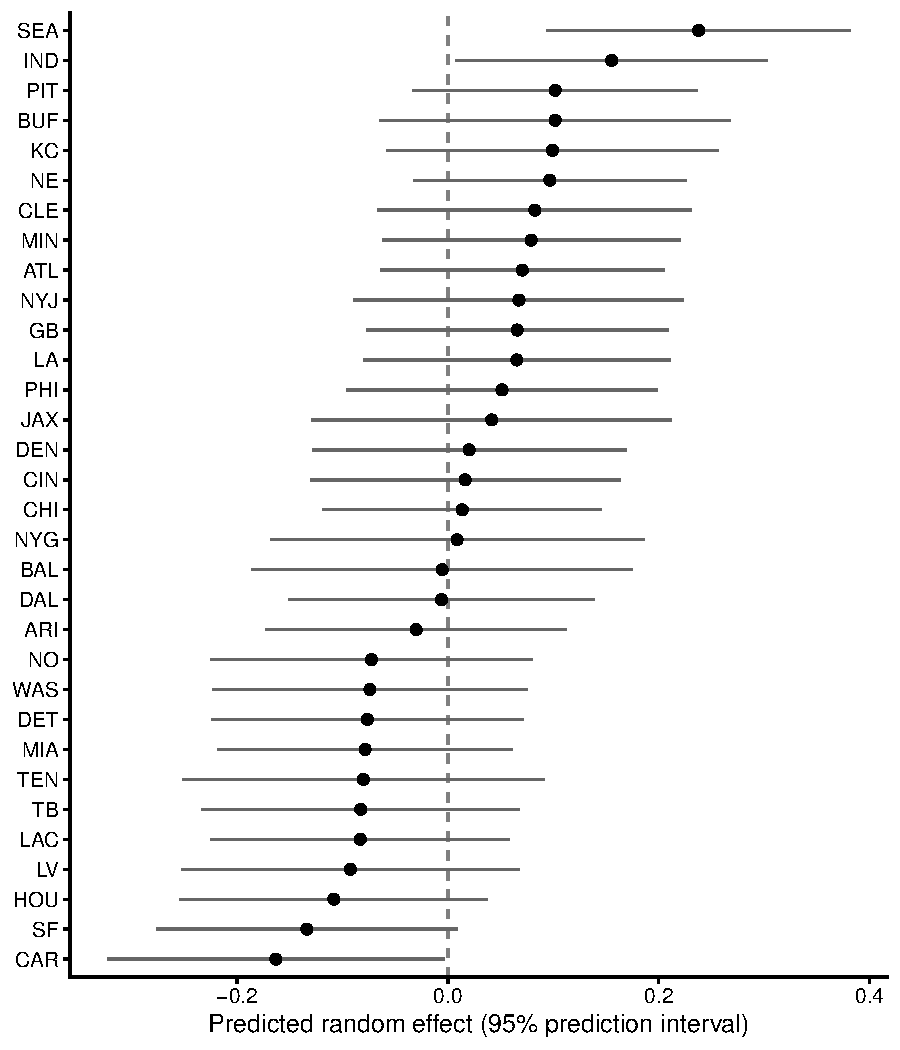
\includegraphics[width= \linewidth]{figures/plots/re_def.pdf}
    \caption{Predicted random effect for each defense. Smaller values correspond to a higher probability of staying in the respective state, i.e., continuing to cover a specific offensive player, and vice versa.}
    \label{fig:re_def}
\end{figure}
%\end{supplement}


\bibliographystyle{oup-abbrvnat}
\bibliography{refs}

\end{document}
